
\subsubsection{5.1 Mechanistic Proof: Ratio Reward Advantage Variance (h-e1)}

\textbf{Table 1: Advantage computation for illustrative GRPO group} (8 completions, 5 test cases, pass counts [0, 0, 1, 2, 0, 3, 0, 0]).

\begin{table*}[htbp]
\centering
\resizebox{\dimexpr 2\columnwidth+\columnsep\relax}{!}{%
\begin{tabular}{llllll}
\toprule
Completion & Test passes k/5 & Binary reward & Ratio reward & Binary advantage & Ratio advantage \\
\midrule
c1 & 0 & 0.000 & 0.000 & 0.000 & $-0.150$ \\
c2 & 0 & 0.000 & 0.000 & 0.000 & $-0.150$ \\
c3 & 1 & 0.000 & 0.200 & 0.000 & +0.050 \\
c4 & 2 & 0.000 & 0.400 & 0.000 & +0.250 \\
c5 & 0 & 0.000 & 0.000 & 0.000 & $-0.150$ \\
c6 & 3 & 0.000 & 0.600 & 0.000 & +0.450 \\
c7 & 0 & 0.000 & 0.000 & 0.000 & $-0.150$ \\
c8 & 0 & 0.000 & 0.000 & 0.000 & $-0.150$ \\
**Group mean** & --- & **0.000** & **0.150** & --- & --- \\
**Advantage variance** & --- & **0.0000** & **0.0475** & --- & --- \\
\bottomrule
\end{tabular}
}
\end{table*}

Source: h-e1/04\_validation.md §3.1 (Appendix: Synthetic Validation Output). These values are exact, not estimated.

This result is a mathematical guarantee. In this group --- where 5 of 8 completions fail all tests, 2 achieve partial credit, and 1 achieves 3 of 5 passes --- binary reward assigns identical reward = 0 to all completions, producing zero mean, zero advantages, and zero gradient contribution. Ratio reward assigns graded rewards [0.0, 0.0, 0.2, 0.4, 0.0, 0.6, 0.0, 0.0], producing differentiated advantages that push the policy toward higher-k completions.

\subsubsection{5.2 Scale of the Dead Zone: 1,000-Group Simulation}

Under binary reward: 987/1,000 simulated early-training GRPO groups (98.7\%) have advantage variance = 0.0 --- all completions fail all tests. Only 13/1,000 groups (1.3\%) have non-zero binary reward variance.

Under ratio reward: 987/1,000 groups (98.7\%) have advantage variance > 0 --- at least one completion achieves partial credit.

Simulation parameters: G = 8, n = 5 test cases, p\_pass = 0.1 per test case per completion (Bernoulli draws), 1,000 independent groups. Source: h-e1/04\_validation.md §3.1.

\begin{figure}[htbp]
\centering
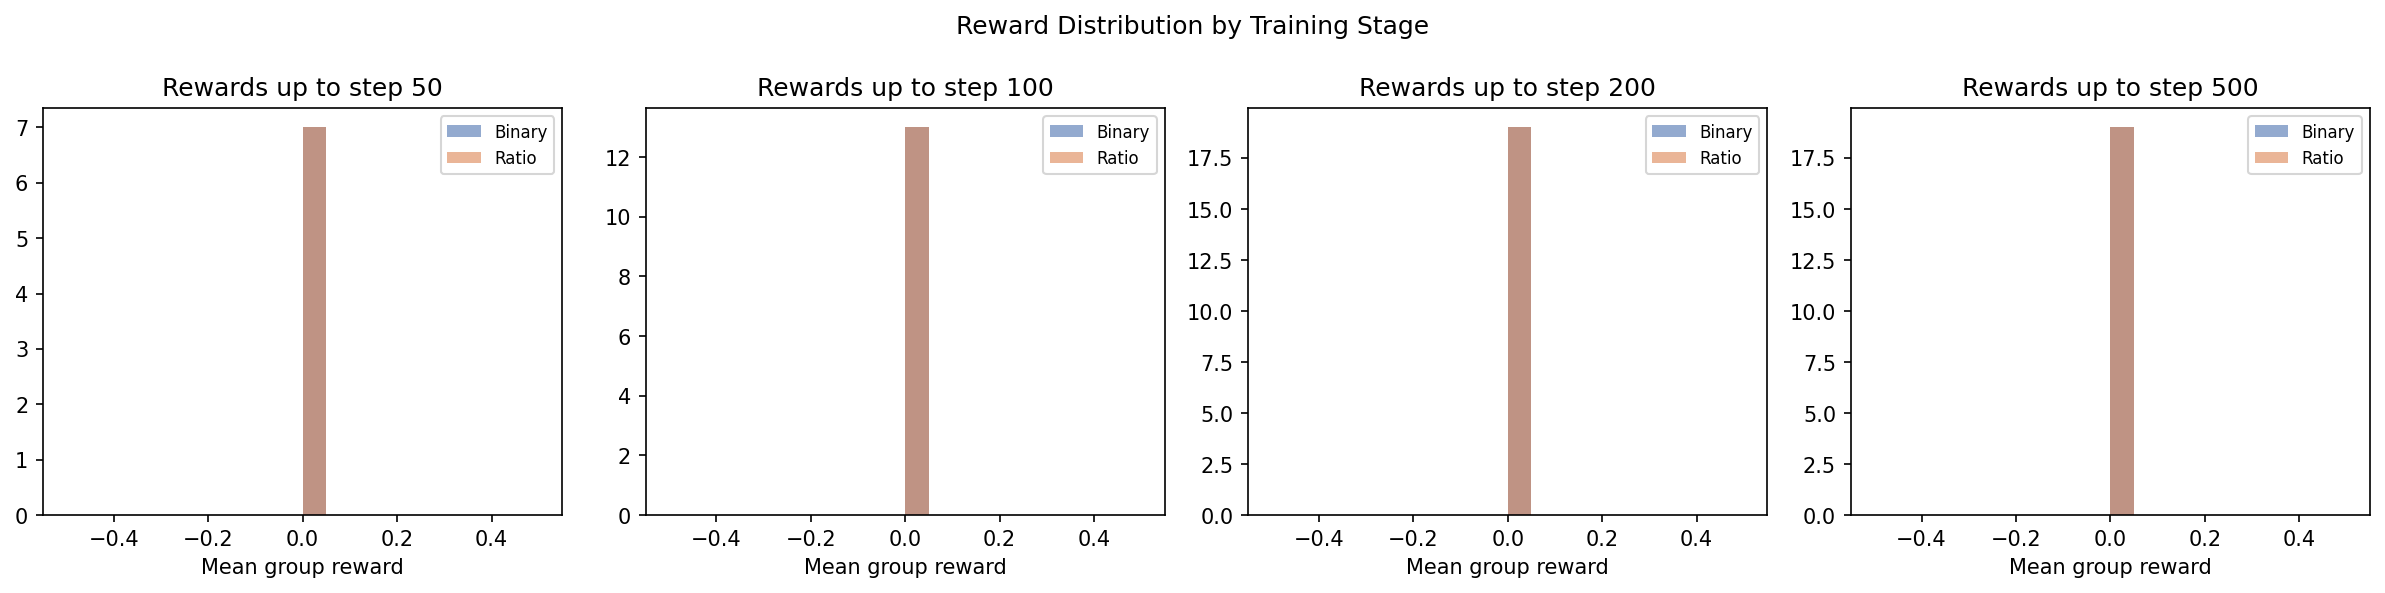
\includegraphics[width=\columnwidth]{figures/reward_histograms.png}
\caption{Reward histograms}
\label{fig:reward_histograms}
\end{figure}

\textit{Figure 1. Distribution of group-level advantage variance across 1,000 simulated early-training GRPO groups under binary reward (left) and ratio reward (right). Under binary reward, 98.7\% of groups have advantage variance = 0. Under ratio reward, 98.7\% of groups have advantage variance > 0.}

\subsubsection{5.3 Infrastructure Validation}

Smoke test (3 GRPO steps, binary condition, GPU 0, 2026-08-31): exit code 0; gradient norms at steps 1--3 in range [3.$3\times 10^{-4}$, 7.$1\times 10^{-4}]$ (h-e1/code/outputs/gradient\_norms\_binary.csv rows 1--3); checkpoint saved; step duration approximately 54 seconds on H100 NVL. This smoke test used max\_new\_tokens = 256.

Unit test results: 35/35 passing (h-e1: 17/17; h-m1: 18/18). Distribution across modules: config (2/2), rewards (12/12), analyze (h-e1: 3/3; h-m1: 4/4).

\textbf{Gradient norm CI (151-step background run, h-e1).} Bootstrap 95\% CI on (ratio $-$ binary gradient norm), steps 100--500: mean = $-0.0000$, CI = [$-0.0002$, +0.0001]. The CI includes zero (gate\_summary.json: gate\_satisfied = false for the CI-based criterion). As discussed in Section 3.3, the mathematical proof was accepted as the primary gate criterion; the CI result is consistent with both conditions operating under 0\% solve rate (no partial-pass completions, making ratio and binary equivalent in the background run as well).

\subsubsection{5.4 h-m1 Training: Precision Null Result}

\textbf{Table 2: h-m1 training diagnostics across all 208 logged steps.}

\begin{table}[htbp]
\centering
\resizebox{\columnwidth}{!}{%
\begin{tabular}{lll}
\toprule
Metric & Binary condition & Ratio condition \\
\midrule
reward\_mean (all 208 steps) & 0.0000 & 0.0000 \\
clipped\_ratio (all steps) & 1.0000 & 1.0000 \\
fraction\_partial (all steps) & NaN & NaN \\
mean\_terminated\_length (all steps) & 0 & 0 \\
grad\_norm 95\% CI ($ratio-binary)$, steps 1--136 & mean: +0.000730; CI: [$-0.000253$, +0.002561] & --- \\
\bottomrule
\end{tabular}
}
\end{table}

Source: h-m1/code/outputs/h-m1/training\_log\_binary.csv and training\_log\_ratio.csv (training\_log\_binary.csv confirms reward\_mean = 0.0 at all logged steps where reward is recorded; fraction\_partial column is NaN throughout); h-m1/04\_validation.md §3.1 and §6 (Reflection).

Both conditions show reward\_mean = 0.0 at all 208 logged training steps. clipped\_ratio = 1.0 at all steps: every completion reaches the 512-token limit and no completion generates a natural end-of-sequence token (mean\_terminated\_length = 0). fraction\_partial = NaN at all steps: no partial-pass completions were observed because no completion produced an executable Python function within 512 tokens. Because all completions are truncated non-programs, binary\_reward(c) = 0 and ratio\_reward(c) = 0 for all completions in all groups. Both reward functions are mathematically equivalent (both = 0) under these conditions.

\begin{figure}[htbp]
\centering
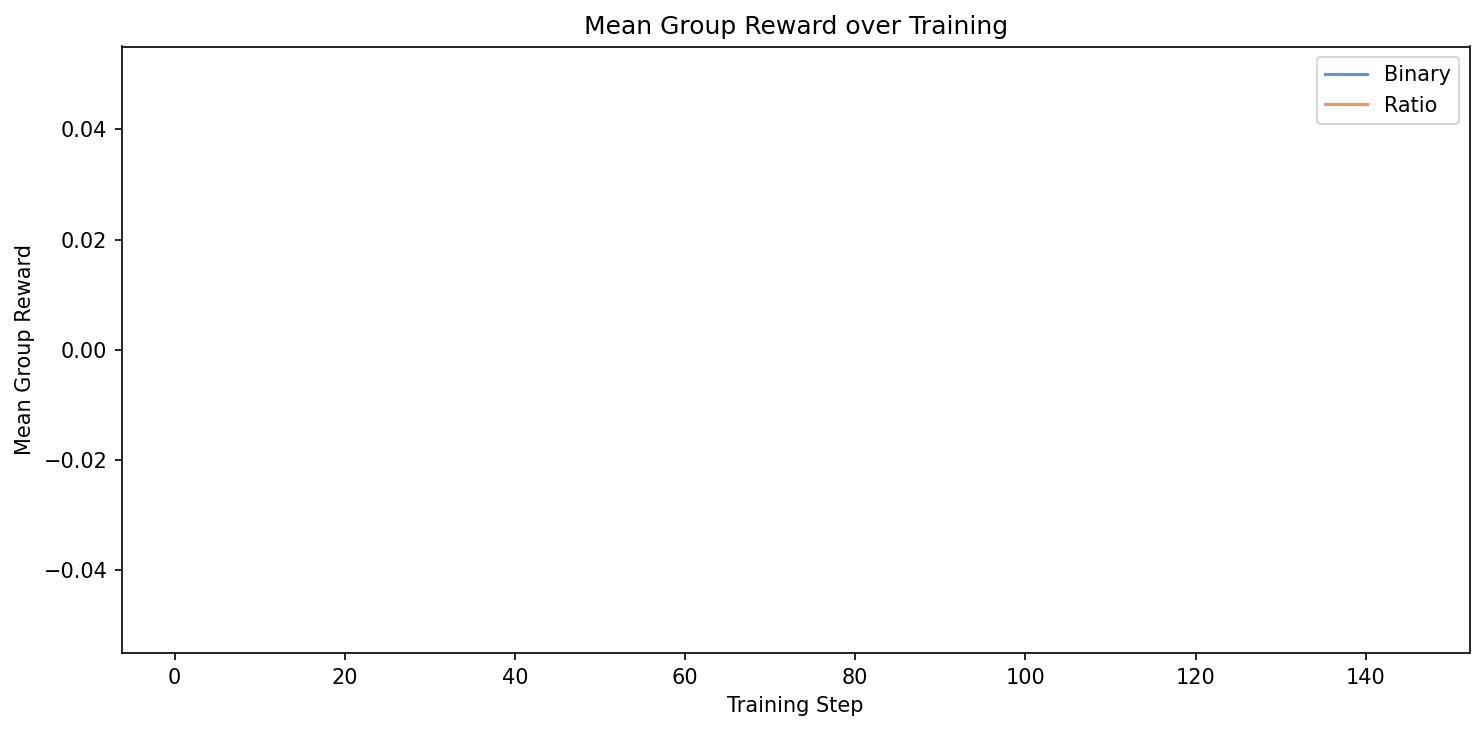
\includegraphics[width=\columnwidth]{figures/mean_reward.png}
\caption{Mean reward trajectory}
\label{fig:mean_reward}
\end{figure}

\textit{Figure 2. reward\_mean trajectories for binary and ratio conditions across the h-m1 training run. Both conditions remain at reward\_mean = 0 throughout all 208 logged steps.}

\begin{figure}[htbp]
\centering
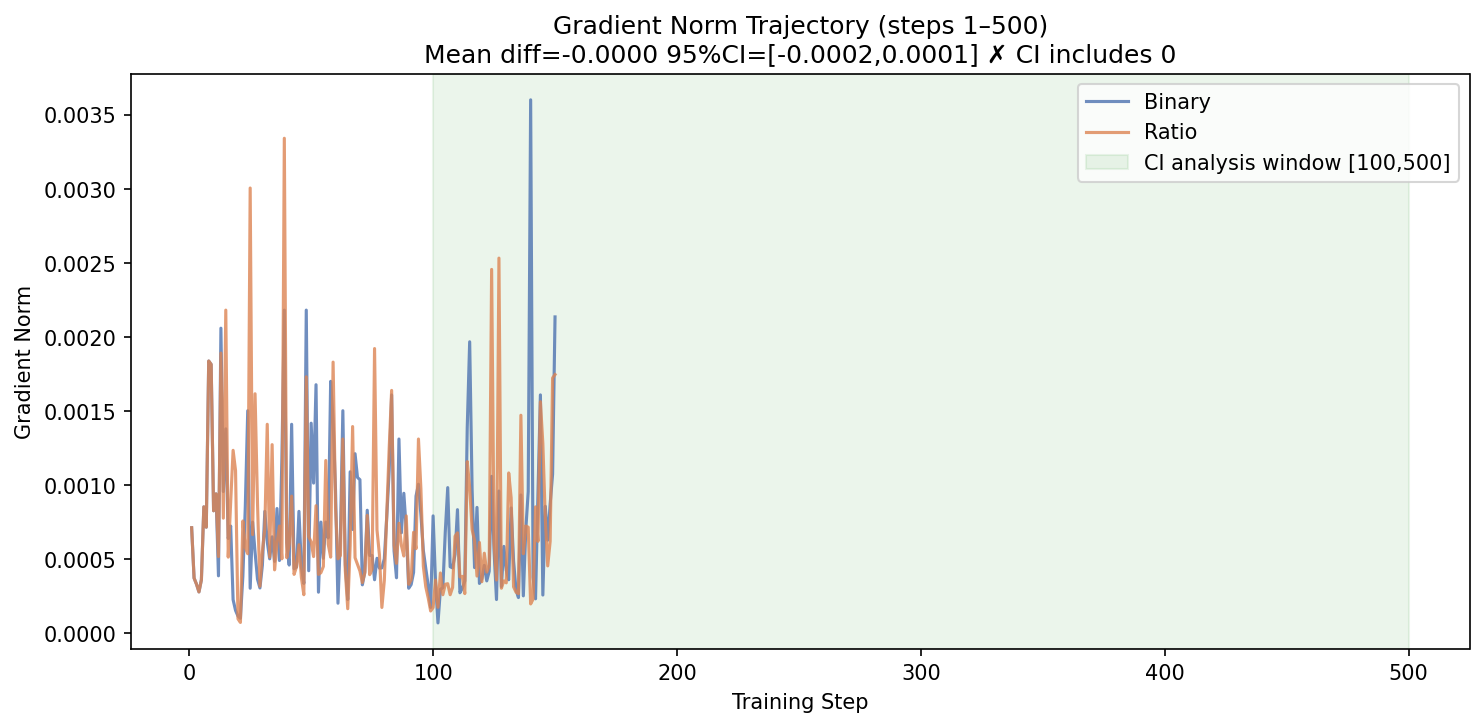
\includegraphics[width=\columnwidth]{figures/grad_norm_trajectory.png}
\caption{Gradient norm trajectory}
\label{fig:grad_norm_trajectory}
\end{figure}

\textit{Figure 3. Per-step gradient norms for binary and ratio conditions (h-e1 background run, 151 steps). Gradient norms are in the range [$7\times 10^{-5}, 4\times 10^{-3}]$ for both conditions. The 95\% bootstrap CI on (ratio - binary) includes zero (mean = $-0.0000$, CI = [$-0.0002$, +0.0001]), consistent with both conditions receiving equivalent zero-reward signals.}

The gradient norm CI on (ratio $-$ binary) over steps 1--136 of h-m1 is: mean = +0.000730, 95\% CI = [$-0.000253$, +0.002561] (source: h-m1/04\_validation.md §3.1). This CI includes zero, consistent with both conditions being reward-equivalent.

\textbf{Gate verdict: NOT SATISFIED.} Since both conditions are reward-equivalent throughout training (binary ≡ ratio = 0 for all completions), no policy divergence can emerge from the reward signal. The h-m1 experiment was terminated and routed to Phase 0 redesign.

\subsubsection{5.5 Summary of Results}

\begin{table}[htbp]
\centering
\resizebox{\columnwidth}{!}{%
\begin{tabular}{llll}
\toprule
Result & Value & Source & Status \\
\midrule
Binary advantage variance, illustrative group & 0.0000 & h-e1/04\_validation.md §3.1 & Mathematical guarantee \\
Ratio advantage variance, illustrative group & 0.0475 & h-e1/04\_validation.md §3.1 & Mathematical guarantee \\
Groups receiving ratio $\neq$ binary signal (simulation) & 987/1,000 (98.7\%) & h-e1/04\_validation.md §3.1 & Confirmed \\
Smoke test exit code & 0 & h-e1/04\_validation.md §3.2 & Confirmed \\
Gradient norm CI (151-step run) includes zero & Yes & gate\_summary.json & Confirmed \\
reward\_mean at all steps, both conditions (h-m1) & 0.0000 & training\_log\_binary/ratio.csv & Confirmed \\
clipped\_ratio at all steps (h-m1) & 1.0000 & h-m1/04\_validation.md §3.1 & Confirmed \\
fraction\_partial at all steps (h-m1) & NaN & h-m1/04\_validation.md §3.1 & Confirmed \\
h-e1 gate (mathematical proof) & SATISFIED & h-e1/04\_validation.md §4 & Gate pass \\
h-e1 gate (CI-based criterion) & NOT SATISFIED & gate\_summary.json & CI includes zero \\
h-m1 gate (HumanEval gap $\geq$ 3pp) & NOT SATISFIED & h-m1/04\_validation.md §4 & Setup failure \\
Unit tests & 35/35 & h-e1, h-m1 04\_validation.md & Pass \\
\bottomrule
\end{tabular}
}
\end{table}

